\documentclass[tikz,border=8pt]{standalone}
\usepackage{amsmath}
\usetikzlibrary{arrows.meta}

\begin{document}
	
	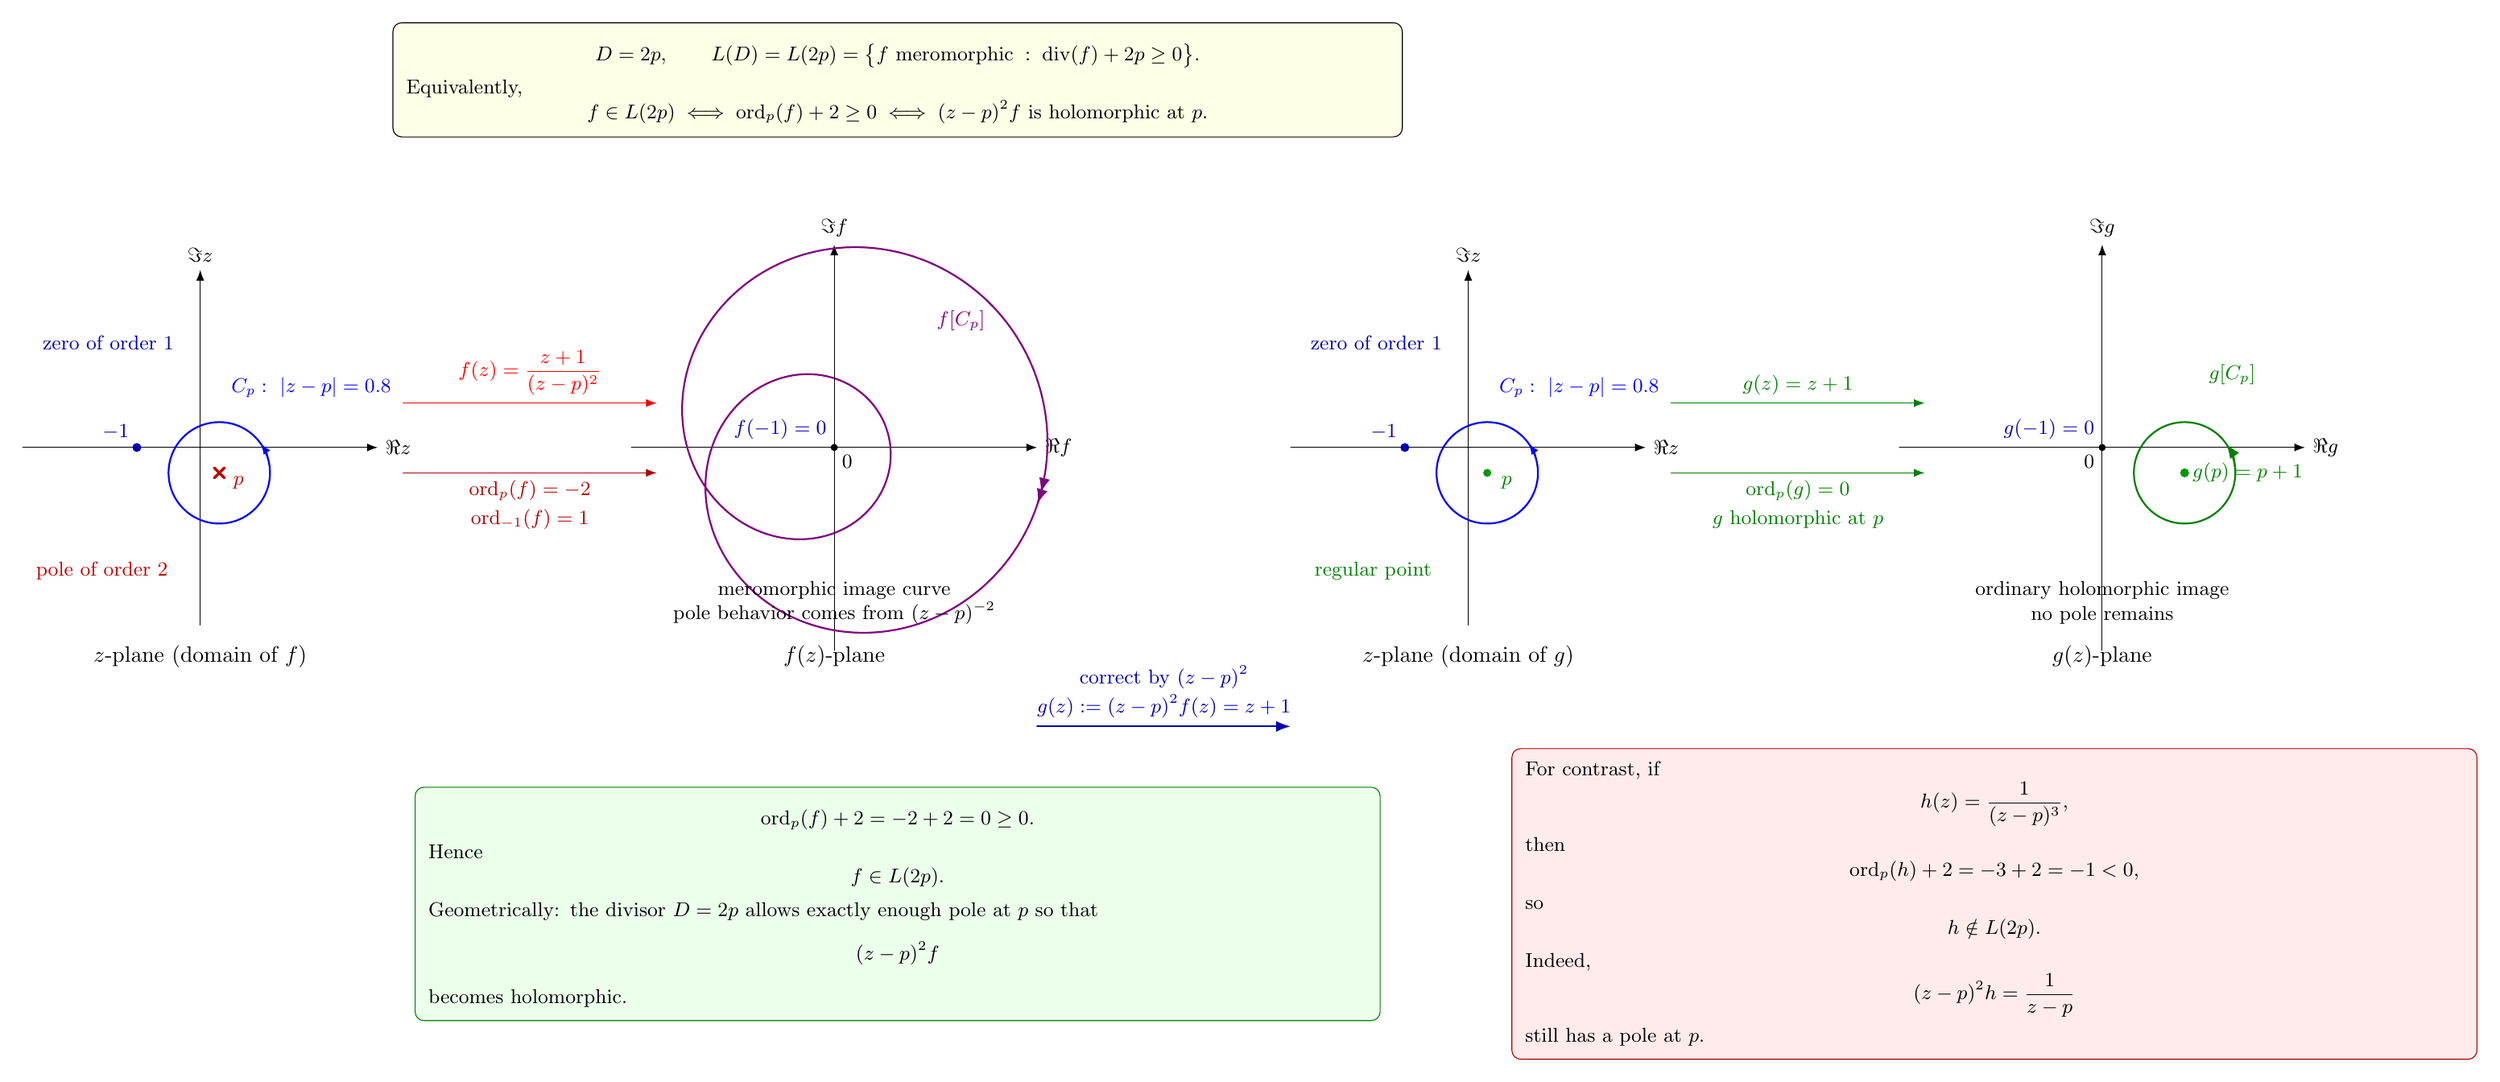
\begin{tikzpicture}[
		>=Latex,
		line cap=round,
		line join=round,
		font=\small,
		x=1cm,y=1cm
		]
		
		%------------------------------------------------
		% Parameters
		%------------------------------------------------
		\def\px{0.3}
		\def\py{-0.4}
		\def\rho{0.8}
		
		\tikzset{
			zero/.style={blue!70!black, fill=blue!70!black},
			polemark/.style={red!75!black, very thick},
			regularpt/.style={green!60!black, fill=green!60!black},
			imgf/.style={violet, thick},
			imgg/.style={green!50!black, thick},
			defbox/.style={draw=black, rounded corners, fill=yellow!10, align=left, inner sep=6pt},
			goodbox/.style={draw=green!50!black, rounded corners, fill=green!8, align=left, inner sep=6pt},
			badbox/.style={draw=red!70!black, rounded corners, fill=red!8, align=left, inner sep=6pt}
		}
		
		%====================================================
		% Top definition box
		%====================================================
		\node[defbox, text width=15.5cm] at (11,-0.2) {%
			\[
			D=2p,\qquad
			L(D)=L(2p)=\bigl\{f\text{ meromorphic}\;:\;\operatorname{div}(f)+2p\ge 0\bigr\}.
			\]
			Equivalently,
			\[
			f\in L(2p)\iff \operatorname{ord}_p(f)+2\ge 0
			\iff (z-p)^2f \text{ is holomorphic at } p.
			\]
		};
		
		%====================================================
		% 1. Domain of f : z-plane
		%====================================================
		\begin{scope}[shift={(0,-6.0)}]
			\node[font=\normalsize] at (0,-3.3) {$z$-plane (domain of $f$)};
			
			% axes
			\draw[->] (-2.8,0)--(2.8,0) node[right] {$\Re z$};
			\draw[->] (0,-2.8)--(0,2.8) node[above] {$\Im z$};
			
			% contour around p
			\draw[blue, thick] (\px,\py) circle (\rho);
			\draw[blue,->] (\px+\rho,\py) arc[start angle=0,end angle=35,radius=\rho];
			\node[blue] at (1.75,0.95) {$C_p:\ |z-p|=\rho$};
			
			% pole p
			\draw[polemark] (\px,\py) ++(-0.08,-0.08) -- ++(0.16,0.16);
			\draw[polemark] (\px,\py) ++(-0.08,0.08)  -- ++(0.16,-0.16);
			\node[red!75!black, right] at (\px+0.10,\py-0.16) {$p$};
			\node[red!75!black] at (-1.55,-1.95) {pole of order $2$};
			
			% zero at z=-1
			\fill[zero] (-1,0) circle (2pt);
			\node[blue!70!black, above left] at (-1,0) {$-1$};
			\node[blue!70!black] at (-1.45,1.65) {zero of order $1$};
		\end{scope}
		
		% Arrow for f
		\draw[->, red] (3.2,-5.3) -- (7.2,-5.3)
		node[midway, above] {$\displaystyle f(z)=\frac{z+1}{(z-p)^2}$};
		
		\draw[->, red!70!black] (3.2,-6.4) -- (7.2,-6.4)
		node[midway, below, align=center] {%
			$\displaystyle \operatorname{ord}_p(f)=-2$\\[2pt]
			$\displaystyle \operatorname{ord}_{-1}(f)=1$};
		
		%====================================================
		% 2. Codomain of f : f-plane
		%====================================================
		\begin{scope}[shift={(10,-6.0)}]
			\node[font=\normalsize] at (0,-3.3) {$f(z)$-plane};
			
			% axes
			\draw[->] (-3.2,0)--(3.2,0) node[right] {$\Re f$};
			\draw[->] (0,-3.2)--(0,3.2) node[above] {$\Im f$};
			
			% origin
			\fill (0,0) circle (1.6pt);
			\node[below right] at (0,0) {$0$};
			\node[blue!70!black, above left] at (0,0) {$f(-1)=0$};
			
			% image curve f(C_p)
			\draw[imgf]
			plot[domain=0:6.283, samples=700]
			(
			{((\px+1+\rho*cos(\x r))*cos(2*\x r) + (\py+\rho*sin(\x r))*sin(2*\x r))/(\rho*\rho)},
			{((\py+\rho*sin(\x r))*cos(2*\x r) - (\px+1+\rho*cos(\x r))*sin(2*\x r))/(\rho*\rho)}
			);
			
			% manual arrows on image curve
			\draw[imgf,->]
			({((\px+1+\rho*cos(0.8))*cos(1.6) + (\py+\rho*sin(0.8))*sin(1.6))/(\rho*\rho)},
			{((\py+\rho*sin(0.8))*cos(1.6) - (\px+1+\rho*cos(0.8))*sin(1.6))/(\rho*\rho)})
			--
			({((\px+1+\rho*cos(0.95))*cos(1.9) + (\py+\rho*sin(0.95))*sin(1.9))/(\rho*\rho)},
			{((\py+\rho*sin(0.95))*cos(1.9) - (\px+1+\rho*cos(0.95))*sin(1.9))/(\rho*\rho)});
			
			\draw[imgf,->]
			({((\px+1+\rho*cos(2.7))*cos(5.4) + (\py+\rho*sin(2.7))*sin(5.4))/(\rho*\rho)},
			{((\py+\rho*sin(2.7))*cos(5.4) - (\px+1+\rho*cos(2.7))*sin(5.4))/(\rho*\rho)})
			--
			({((\px+1+\rho*cos(2.85))*cos(5.7) + (\py+\rho*sin(2.85))*sin(5.7))/(\rho*\rho)},
			{((\py+\rho*sin(2.85))*cos(5.7) - (\px+1+\rho*cos(2.85))*sin(5.7))/(\rho*\rho)});
			
			\node[violet] at (2.0,2.0) {$f[C_p]$};
			\node[align=center] at (0,-2.45) {meromorphic image curve\\pole behavior comes from $(z-p)^{-2}$};
		\end{scope}
		
		%====================================================
		% Correction arrow
		%====================================================
		\draw[->, blue!70!black, thick] (13.2,-10.4) -- (17.2,-10.4)
		node[midway, above, align=center] {%
			$\displaystyle \text{correct by }(z-p)^2$\\[2pt]
			$\displaystyle g(z):=(z-p)^2f(z)=z+1$};
		
		%====================================================
		% 3. Domain of g : z-plane again
		%====================================================
		\begin{scope}[shift={(20,-6.0)}]
			\node[font=\normalsize] at (0,-3.3) {$z$-plane (domain of $g$)};
			
			% axes
			\draw[->] (-2.8,0)--(2.8,0) node[right] {$\Re z$};
			\draw[->] (0,-2.8)--(0,2.8) node[above] {$\Im z$};
			
			% same contour
			\draw[blue, thick] (\px,\py) circle (\rho);
			\draw[blue,->] (\px+\rho,\py) arc[start angle=0,end angle=35,radius=\rho];
			\node[blue] at (1.75,0.95) {$C_p:\ |z-p|=\rho$};
			
			% p becomes regular
			\fill[regularpt] (\px,\py) circle (1.8pt);
			\node[green!50!black, right] at (\px+0.10,\py-0.16) {$p$};
			\node[green!50!black] at (-1.5,-1.95) {regular point};
			
			% zero at z=-1
			\fill[zero] (-1,0) circle (2pt);
			\node[blue!70!black, above left] at (-1,0) {$-1$};
			\node[blue!70!black] at (-1.45,1.65) {zero of order $1$};
		\end{scope}
		
		% Arrow for g
		\draw[->, green!50!black] (23.2,-5.3) -- (27.2,-5.3)
		node[midway, above] {$\displaystyle g(z)=z+1$};
		
		\draw[->, green!50!black] (23.2,-6.4) -- (27.2,-6.4)
		node[midway, below, align=center] {%
			$\displaystyle \operatorname{ord}_p(g)=0$\\[2pt]
			$\displaystyle g \text{ holomorphic at }p$};
		
		%====================================================
		% 4. Codomain of g : g-plane
		%====================================================
		\begin{scope}[shift={(30,-6.0)}]
			\node[font=\normalsize] at (0,-3.3) {$g(z)$-plane};
			
			% axes
			\draw[->] (-3.2,0)--(3.2,0) node[right] {$\Re g$};
			\draw[->] (0,-3.2)--(0,3.2) node[above] {$\Im g$};
			
			% origin
			\fill (0,0) circle (1.6pt);
			\node[below left] at (0,0) {$0$};
			\node[blue!70!black, above left] at (0,0) {$g(-1)=0$};
			
			% center g(p)=p+1
			\fill[regularpt] (\px+1,\py) circle (2pt);
			\node[green!50!black, right] at (\px+1,\py) {$g(p)=p+1$};
			
			% image circle
			\draw[imgg] ({\px+1},{\py}) circle (\rho);
			\draw[imgg,->] ({\px+1+\rho},{\py}) arc[start angle=0,end angle=35,radius=\rho];
			
			\node[green!50!black] at (2.05,1.15) {$g[C_p]$};
			\node[align=center] at (0,-2.45) {ordinary holomorphic image\\no pole remains};
		\end{scope}
		
		%====================================================
		% Membership box
		%====================================================
		\node[goodbox, text width=14.8cm] at (11,-13.2) {%
			\[
			\operatorname{ord}_p(f)+2=-2+2=0\ge 0.
			\]
			Hence
			\[
			f\in L(2p).
			\]
			Geometrically: the divisor \(D=2p\) allows exactly enough pole at \(p\) so that
			\[
			(z-p)^2f
			\]
			becomes holomorphic.};
		
		%====================================================
		% Optional contrast box
		%====================================================
		\node[badbox, text width=14.8cm] at (28.3,-13.2) {%
			For contrast, if
			\[
			h(z)=\frac{1}{(z-p)^3},
			\]
			then
			\[
			\operatorname{ord}_p(h)+2=-3+2=-1<0,
			\]
			so
			\[
			h\notin L(2p).
			\]
			Indeed,
			\[
			(z-p)^2h=\frac{1}{z-p}
			\]
			still has a pole at \(p\).};
		
	\end{tikzpicture}
	
\end{document}